\documentclass[a4paper,12pt]{book}
\usepackage{amsmath, amsthm}
\usepackage{datetime}
\usepackage{framed}
\usepackage{enumitem}
\usepackage{fancyref}
\usepackage{wrapfig}
\usepackage{pifont}
\usepackage{appendix}
\usepackage{caption}
\usepackage{xcolor}
\usepackage[stable]{footmisc}
\usepackage{multicol}
\usepackage{csquotes}
\usepackage{pdfpages}

\usepackage{amsthm}

\usepackage{amssymb}
\usepackage{amsfonts}
\usepackage{mathtools}

\usepackage{eso-pic}
\usepackage{tikz}
\usepackage{pgf}
\usepgflibrary{fpu}
\usepackage{qtree}
\usetikzlibrary{angles,fit,arrows,calc,math,intersections,through,backgrounds,cd}
\usepackage{pgfplots}
\usepackage{tkz-euclide}

\usepackage{listings}
\lstset{
    basicstyle=\itshape,
    xleftmargin=3em,
    literate={->}{$\rightarrow$}{2}
{α}{$\alpha$}{1}
{δ}{$\delta$}{1}
}


\usepackage{csquotes}
\renewcommand{\mkbegdispquote}[2]{\itshape}

\newdateformat{nianyueri}{修订于 \THEYEAR 年 \THEMONTH 月 \THEDAY 日 }


\usepackage{quiver}
\usepackage{circledsteps}
\usepackage[top=1in,bottom=1in,left=1in,right=1in]{geometry} % 用于设置页面布局
\usepackage{xeCJK} % 用于使用本地字体
\usepackage[super, square, sort&compress]{natbib} % 处理参考文献
\usepackage{titlesec, titletoc} % 设置章节标题及页眉页脚
\usepackage{amssymb}
\usepackage{amsmath} % 在公式中用\text{文本}输入中文
\usepackage{diagbox}
\usepackage{multirow} % 表格中使用多行
\usepackage{booktabs} % 表格中使用\toprule等命令
\usepackage{rotating} % 使用sidewaystable环境旋转表格
\usepackage{tabularx}
\usepackage{graphicx} % 处理图片
\usepackage{footnote} % 增强的脚注功能,可添加表格脚注
\usepackage{threeparttable} % 添加真正的表格脚注,示例见README
\usepackage{hyperref} % 添加pdf书签

\usepackage{tikz}
\usetikzlibrary{shapes,arrows,shadows}


% 字体设置
\setmainfont{Times New Roman}
\setsansfont[Scale=MatchLowercase,Mapping=tex-text]{PT Sans}
\setmonofont[Scale=MatchLowercase]{PT Mono}
\setCJKmainfont[ItalicFont={FZKai-Z03}, BoldFont={FZHei-B01}]{FZShuSong-Z01}
\setCJKsansfont{FZHei-B01}
\setCJKmonofont{FZShuSong-Z01}

\newcommand{\song}{\CJKfamily{song}} % 宋体
\newcommand{\fs}{\CJKfamily{fs}} % 仿宋体
\newcommand{\kai}{\CJKfamily{kai}} % 楷体
\newcommand{\hei}{\CJKfamily{hei}} % 黑体
\newcommand{\li}{\CJKfamily{li}} % 隶书
\newcommand{\you}{\CJKfamily{you}} % 幼圆
\def\songti{\song}
\def\fangsong{\fs}
\def\kaishu{\kai}
\def\heiti{\hei}
\def\lishu{\li}
\def\youyuan{\you}

%%设置常用中文字号,方便调用
\newcommand{\chuhao}{\fontsize{42pt}{\baselineskip}\selectfont}
\newcommand{\xiaochu}{\fontsize{36pt}{\baselineskip}\selectfont}
\newcommand{\yihao}{\fontsize{26pt}{\baselineskip}\selectfont}
\newcommand{\xiaoyi}{\fontsize{24pt}{\baselineskip}\selectfont}
\newcommand{\erhao}{\fontsize{22pt}{\baselineskip}\selectfont}
\newcommand{\xiaoer}{\fontsize{18pt}{\baselineskip}\selectfont}
\newcommand{\sanhao}{\fontsize{16pt}{\baselineskip}\selectfont}
\newcommand{\xiaosan}{\fontsize{15pt}{\baselineskip}\selectfont}
\newcommand{\sihao}{\fontsize{14pt}{\baselineskip}\selectfont}
\newcommand{\xiaosi}{\fontsize{12pt}{\baselineskip}\selectfont}
\newcommand{\wuhao}{\fontsize{10.5pt}{\baselineskip}\selectfont}
\newcommand{\xiaowu}{\fontsize{9pt}{\baselineskip}\selectfont}
\newcommand{\liuhao}{\fontsize{7.5pt}{\baselineskip}\selectfont}
\newcommand{\xiaoliu}{\fontsize{6.5pt}{\baselineskip}\selectfont}
\newcommand{\qihao}{\fontsize{5.5pt}{\baselineskip}\selectfont}
\newcommand{\bahao}{\fontsize{5pt}{\baselineskip}\selectfont}

% 章节标题显示方式及页眉页脚设置
% \item xCJKnumb是自己额外安装的包
% \item titleformat命令定义标题的形式
% \item titlespacing定义标题距左、上、下的距离
\titleformat{\section}{\raggedright\large\bfseries}{\thesection}{1em}{}
\titleformat{\subsection}{\raggedright\normalsize\bfseries}{\thesubsection}{1em}{}
\titlespacing{\section}{0pt}{*2}{*0}
\titlespacing{\subsection}{0pt}{*1}{*0}

% 由于默认的2em缩进不够,所以我手动调整了,但是在windows下似乎2.2就差不多了,或者是article中没有这个问题
\setlength{\parindent}{0em}
\setlength{\parskip}{0.25em}

% 设置表格标题前后间距
\setlength{\abovecaptionskip}{0pt}
\setlength{\belowcaptionskip}{0pt}

% 设置列表项目前后间距
\setlength\itemsep{0em}

\renewcommand{\refname}{\bfseries{参~考~文~献}} %将Reference改为参考文献(用于 article)
% \renewcommand{\bibname}{参~考~文~献} %将bibiography改为参考文献(用于 book)

\renewcommand{\baselinestretch}{1.4} %设置行间距
\renewcommand{\figurename}{\small\ttfamily 图}
\renewcommand{\tablename}{\small\ttfamily 表}


\usepackage{stmaryrd}
\usepackage{mathtools}
\usepackage{wasysym}
\usepackage{textcomp}
\usepackage{blindtext}
\usepackage{subfiles}

\newtheorem{problem}{问题}
\numberwithin{problem}{section}
\newtheorem{definition}{定义}
\numberwithin{definition}{section}
\newtheorem{lemma}{引理}
\numberwithin{lemma}{section}
\newtheorem{proposition}{命题}
\numberwithin{proposition}{section}
\newtheorem{theorem}{定理}
\numberwithin{theorem}{section}
\newtheorem{grammar}{文法}
\numberwithin{grammar}{section}
\newtheorem{program}{程序}
\numberwithin{program}{section}
\newtheorem{convention}{约定}
\numberwithin{convention}{section}
\newtheorem{corollary}{推论}
\numberwithin{corollary}{section}
\renewcommand*{\proofname}{证明}

\xeCJKsetwidth{‘’“”}{1em}

\title{来自算术表达式几何的邀请}
\date{\nianyueri\today}
\author{苑明理}

\begin{document}

\begin{titlepage}
\AddToShipoutPictureBG*{%
\AtPageLowerLeft{%
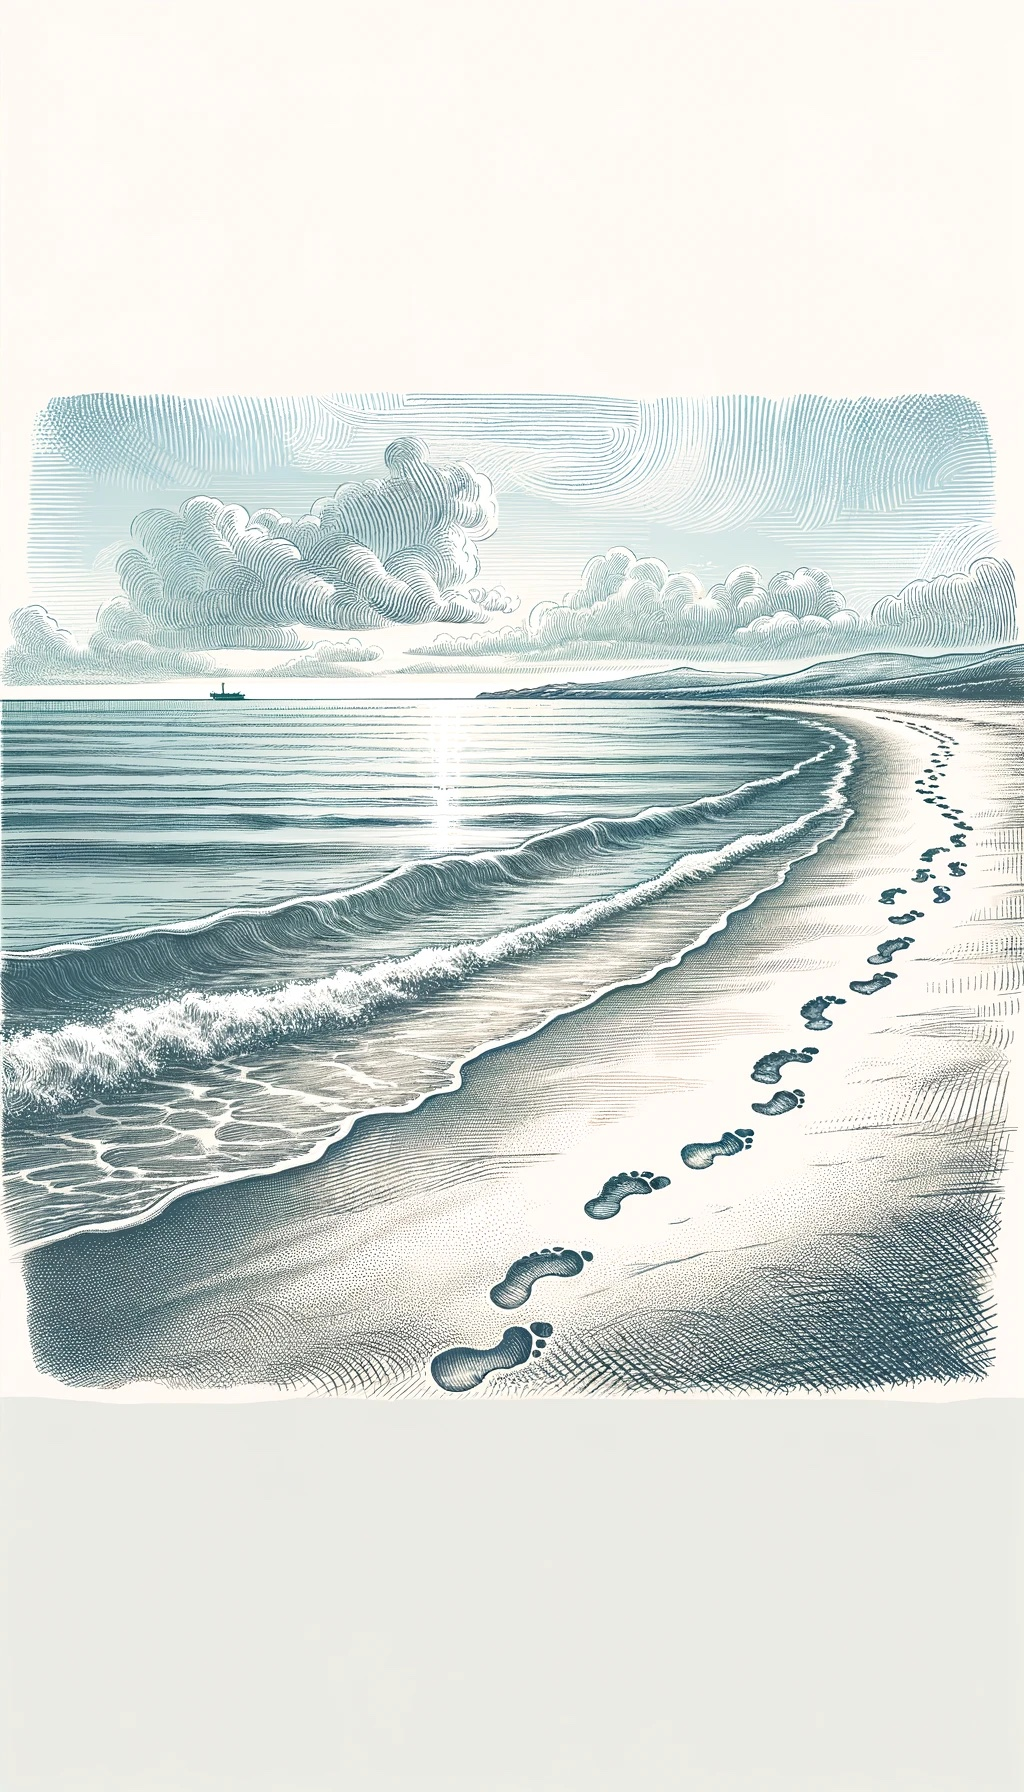
\includegraphics[width=\paperwidth,height=\paperheight]{../images/seaside-footprints.jpg}%
}%
}

\centering{\erhao 来自算术表达式几何的邀请}\\
\vspace{10mm}
\vspace{\fill}
\centering{\sihao 苑明理 \\ \wuhao 修订于 2024 年 3 月 18 日}
\end{titlepage}

\newpage
\thispagestyle{empty}

\frontmatter
\thispagestyle{empty}

\newpage
\thispagestyle{empty}
\vspace*{2cm}
\begin{center}
\parbox{10cm}{\wuhao \em 我们在未知的海岸边发现了一串奇怪的脚印......\flushright— 亚瑟·爱丁顿}
\end{center}

\newpage
\thispagestyle{empty}

\centerline{\rule{13cm}{0.4pt}}
\renewcommand{\contentsname}{\hfill\bfseries 目录\hfill}
\setcounter{tocdepth}{2}
\tableofcontents
\centerline{\rule{13cm}{0.4pt}}

\mainmatter

\chapter{序言}

我深知自己智力和能力的有限,然而当你面对浮现出来的这些有趣问题时,当你感觉到这些问题背后可能的前景时,你是否会选择远航出发,去探索一片未知的海域?
我在 2022 年初的选择是“出发”。尽管这篇文档的每一节都有许多问题没有解决,经过两年多的整理和探索,我逐步可以用相对严格的语言来陈述这些问题了。
所以,我想邀请大家一起来探索这片未知的海域。这个演示文档是我对这个领域的一个简要介绍,希望能够引起大家的兴趣,也多少奢望能够得到指导、指正和帮助。

\newpage

\chapter{故事的开端}

我们的探索大概可以从 2013 年开始讲起。当时,自然语言处理里有一种词嵌入技术被发展出来,引发了大量的研究与讨论。
它最吸引人的地方在于这种分布式表征的词向量,可以捕捉到词语之间的语义关系,被称为“正则性”(regularity)。
正则性是指,如果两对词语在语义关系上有相似性,那么它们的词向量之间的关系也有几何上的平行性。
正则性是词语关系的一种几何化表达,它是词向量的一个重要性质。

![页三](/curiosity/invitation/003.jpeg)

最为著名的例子是“男人”和“女人”之间的关系,与“国王”和“王后”之间的关系。这两对词语之间的关系是相似的,所以它们的词向量之间的关系也应该是平行的。
在上图的例子中,我们可以看到两组平行关系:

* 性别维度移动:男人 - 女人 ≈ 国王 - 女王
* 王权维度移动:国王 - 男人 ≈ 女王 - 女人

这两组关系之间的平行性,形成一个平行四边形。同时,这两组平行关系也可以看成一种关系矢量上的运算,用几何语言说就是:

* 男人 + 性别维度移动 + 王权维度移动 = 女王
* 男人 + 王权维度移动 + 性别维度移动 = 女王

也就是说:

* 性别维度移动 + 王权维度移动 = 王权维度移动 + 性别维度移动

这反映了关系运算的交换律。

当时的算法对这种关系正则性的捕捉是有限的,以后的技术发展也没有沿着这个方向继续前进,而是转向了更加复杂的模型和任务。我思考的起点就恰恰是从这里延伸出来的。
如果我们把这种关系正则性强制要求下来,会发生什么呢?

2015 年的秋天,我去拿数字和数字的运算关系做了一些尝试,但很快就发现它存在一些困难。

![页四](/curiosity/invitation/004.jpeg)

这个困难可以表述为两点:运算关系不具备交换性,从而无法形成平行四边形;欧式空间的容量是有限的,无法容纳指数爆炸的运算关系组合。
让我们举例子来说明一下,我们考察简单的“+1”和“x2”的关系。此时,所有的数字都映射为空间的点,而“+1”和“x2”运算关系映射为空间的向量。

从一个点 $\alpha$ 出发,我们可以进行一系列的运算关系组合,比如:
* 先“+1”再“x2”操作:$(\alpha +1) \times 2 = 2 \alpha + 2$
* 先“x2”再“+1”操作:$\alpha \times 2 + 1 = 2 \alpha + 1$

不论我们从哪个点出发,这两个运算关系都不具备交换性,所以它们无法形成平行四边形。
平行四边形的存在也意味着两次关系运算的组合中可以约化掉一个,从而可以避免运算关系组合的指数爆炸。
而关系不具备交换性,平行四边形就无法形成,指数爆炸的运算关系组合也就无法避免。

如果每个特征在表征空间里都占据有限大的体积,且这个有限大的体积存在一个最小的分辨限制,那么组合爆炸就意味着我们需指数增长的体积来容纳这些运算关系的组合。
在欧式空间里,球体的体积随着半径增长是多项式级别增长的,所以随着表达式数量的增加,表征空间会很快不足够使用。

幸运的是,几何学里有一种空间,它的容量是指数增长的,同时它里面也不存在平行四边形构造,这就是双曲空间。我决定拿双曲空间来尝试解决这个问题。

![页五](/curiosity/invitation/005.jpeg)

经过一些尝试,我很快就发现,一种称之为四阶无限边形铺嵌的结构可以用来编码一些数字的加法和乘法。如上图,横着的最主要的那根轴是加法轴,数字按照加法的规律从左到右不断加一排布;
与之垂直的轴是乘法轴,数据按照乘法的规律逐步乘二排布。与乘法轴垂直的都是加法轴,而与加法轴垂直的都是乘法轴。通过这种加乘交错的构造我们可以编码数字的加法和乘法运算。

当这个数字的四阶无限边形排布做出来以后,望着这些高度对称分布的点值,我产生了非常自然的一个疑问和推测,这些离散点值能否连续扩展到整个庞加莱圆盘?
如果这些点值能连续的分布在整个庞加莱圆盘上,那么我们就可以用它来编码所有实数值的算术运算了。
此后,我就一直在业余时间对相关的问题进行探索,陆陆续续有了一些收获。但这个最初的问题,我至今还没有完全解决。
有朋友告诉我,它可能和一些复杂的模函数有关系。

时间飞逝到了 2019 年,我在出差的飞机上,突然想到既然我希望这些点值能够连续的分布在整个庞加莱圆盘上,那么为什么我不试一下无穷小的生成过程呢?
我在飞机上快速做了一些推导,结果是正面的。旅途结束后的几天,我就得到了一个微分方程,它描述了一个加法和乘法的双生成元的无穷小生成过程。

![页八](/curiosity/invitation/008.jpeg)

整个推导非常初等,只是极限过程和微元的基本运算。因为这个方程刻画了一个计算的流动过程,所以我称之为“流方程”。

![页九](/curiosity/invitation/009.jpeg)

流方程是可解的,解刻画了一个连续生成过程,再稍微分析一下就可以发现这个连续生成过程里容纳一个离散生成过程,刚好对应前面双曲圆盘里的四阶无限边形结构。
这一点我们会在后面的章节里详细讨论。

2021 年春天,我得到公司(彩云科技)的支持,和两个实习生一起工作了三个月,做了一些更加严谨的研究。来自山东大学的张乐同学利用分离变量法很快推导出了一个流方程的解析解。

![页六](/curiosity/invitation/006.jpeg)

在这个解析解之前,我们仅有一些猜测,比如庞加莱圆盘里的四阶无限边形结构,它只是知道离散结构,但不知道连续结构。
而张乐给出的解析解,让我们第一次有了一个可以仔细研究的严格数学对象。我经过一些尝试,画出了这个解析解的图像,发现它的离散生成关系,
和一种称为 Baumslag–Solitar 群的生成关系是一致的,于是也就有了上图。

![页七](/curiosity/invitation/007.jpeg)

在上图中,我们首先可以看到一些红色的离散点值$a$,它们符合解析式 $a = -\frac{x}{y}$。
蓝横线是伪圆,它们从右向左按照加一的规律不断增长,代表了一条条的加法轴。 绿竖线是测地线,它们从上向下按照乘二的规律不断增长,代表了一条条的乘法轴。
蓝横线和绿竖线交错排布,彼此垂直。

因为蓝横线和绿竖线交错的网格的存在,我们可以利用它来编码一些数值的算术运算。比如 $1 \times 8 - 5 = 3$,我们可以在网格上画出这个算术运算的路径。
从任何一个 $a$ 值为 $1$ 的点出发,向下走三步,完成三次乘二操作,然后向右走五步,完成减五的操作,就会到达一个 $a$ 值为 $3$ 的点,也就是上图中黑色的线。

完全类似的,上图中紫红色的线编码了 $(1 - \frac{5}{8}) \times 8 = 3$ 的算术运算;
褐色的线编码了 $(((1 - \frac{1}{8}) \times 2 - \frac{2}{4}) \times 2 - 1) \times 2 = 3$ 的算术运算。

上面的例子都是折线,那么有趣的问题是橙色的曲线编码了什么?仔细考虑一下,就会意识到它编码了一种特别的、不同于传统的黎曼积分的积分过程。黎曼积分只是累加小量;
而这个曲线代表的积分过程会同时累加小量和累乘小量,加法的小量是指趋近于零的量,而乘法的小量是指趋近于一的量。

\newpage

\chapter{基本概念}

本节我们作更加严格的讨论,引入一些基本概念,然后展示一些示例性的算术表达式空间。

算术表达式

从计算机科学的角度来看,算术表达式是一种抽象的递归数据类型,它可以被解析成为一棵树。这棵树的叶子节点是操作数,内部节点是操作符。
所以也可以说,算术表达式有字串表示和树表示两种形式,常见的形式是字串表示,基于中缀表示法和括号的优先级规则。

![页十一](/curiosity/invitation/011.jpeg)

我们尝试在有理数域 $Q$ 上给出算术表达式的定义。这是一种生成式的递归定义方式,它说明:
* 有理数本身就构成算术表达式
* 算术表达式的加、减、乘、除组合仍然构成算术表达式

纯数学专业的读者可能会不熟悉这种定义方式,可以参考形式语言里的生成式定义,我们这里终止符号是有理数、括号和四则运算符号。

![页十二](/curiosity/invitation/012.jpeg)

在这个递归生成结构上也可以递归定义一个求值的过程,可以理解成表达式树表示上的一种遍历过程。一般来讲,这个遍历的求值过程不唯一。
但是同一个表达式树的求值结果是唯一的。

![页十三](/curiosity/invitation/013.jpeg)

然而有一些算术表达式的求值过程是唯一的,比如下图展示的向左或者向右展开的可线索化表达式。
可线索化表达式是指一类算术表达式,它的左支或者右支全部都是叶节点。这种表达式的求值过程是唯一的。向左或者向右展开完全是对称的,
向左展开的形式在求值时是从头计算到尾,向右展开的形式在求值时是从尾计算到头。这里我们取向左展开作为标准形式。

![页十四](/curiosity/invitation/014.jpeg)

细心的读者可能已经注意到,我们的算术表达式时是定义在有理数域上的,为什么不能直接定义在实数域呢。原因是我们在定义表达式的除法时,必须要求除数不为零。
而在有理数域上,一个子表达式是否为零是可以判定的。在实数域上,表达式是否为零不可判定的。为了使概念的定义完整,我们先把算术表达式定义在有理数域上。
然后再通过适当的完备化的手法,把它推广到实数域上。这里有理数域的选择,其实反映了语法与语义的差别。我们算术表达式的递归定义是纯粹的语法式的,
为了回避语义上的困难,我们不得不选择有理数域。

![页十五](/curiosity/invitation/015.jpeg)

下面我们讨论算术表达式的离散生成关系如何做成群的。我们引入离散的加法和乘法生成元,在自由生成下,可以得到一个表达式上的群结构(注意是表达式上的,不是值上的群结构)。
这个过程在几何上得到一些由特定正交线族上的折线构成的路径,这为后继的讨论提供了第一步的基础。

![页十六](/curiosity/invitation/016.jpeg)

下面考察这个自由群的交换子,交换子刻画了群的不可交换性。这里我们考察生成元构成的交换子,如下有几种不同的引进方式。
我们把第三种方式称为“算术扭曲”,因为直观上,这种加法和乘法上的不可交换性,造成了几何空间的扭曲。
需要指出,因为生成元带来的运算被解释为几何上的路径,那么算术扭曲也是一种定义在几何路径上的量。

![页十七](/curiosity/invitation/017.jpeg)

流方程

和前一节讨论的有理数域上的表达式不同,在那里我们做了准备和铺垫,希望通过完备化来构造出算术表达式的几何空间。这是一种构造性的途径和研究方法。
本节则有所不同,我们在这里使用微积分的工具,直接在几何空间上讨论一个标量场$a$,称为赋值场,这个场满足流方程,可以证明前一小节讨论的离散路径群结构可以嵌入到这个几何图景里。
这两种不同的途径都是我们研究的工具。

![页十九](/curiosity/invitation/019.jpeg)

我们在最初引入流方程的时候,使用的是局部极坐标系;类似,我们也可以引入对应的局部笛卡尔坐标系;甚至,我们也可以推导出梯度线-等值线坐标系。
在这些坐标系里,流方程有不同的形式,但是它们都是等价的。这是因为流方程是赋值场 $a$ 的局部性质,它本身不依赖于坐标系的选择。

![页二十](/curiosity/invitation/020.jpeg)

这些局部的坐标系可以刻画赋值场 $a$,同样也可以通过第一基本形式来刻画几何空间本身。我们需要指出,
这些局部刻画需要一个全局的适配条件才能拼接成一个整体的刻画。

形式上,流方程是可以解出来的,不同坐标系下的解会带给我们不同的几何图景。

![页二一](/curiosity/invitation/021.jpeg)

局部极坐标系下的解,我们通过泰勒展开、变形、引入倍角公式的处理,最终得到了一个公式。
仔细观察这个公式会发现,它在 $\theta$ 角取值为 $0$、$\frac{\pi}{2}$、$\pi$、$\frac{3\pi}{2}$ 时,分别编码了加减乘除四种运算。
如此,我们就可以把算术表达式离散生成的群结构作为路径嵌入到这个几何空间里。

![页二二](/curiosity/invitation/022.jpeg)

局部梯度线-等值线坐标系下的流方程也是可解的。对于以 $0$ 值为起点的情形,我们发现此时的解和双曲空间中圆的周长公式形式是一样的,只差一个比例系数。
这给我们带来了一种扩散圆的几何图景,扩散圆的周长乘以某个比值就是赋值场。
直观上,当有多个零点或者零点构成零线时,我们使用惠更斯原理,用这些扩散圆的叠加,也就是波前来刻画赋值场。
目前这个几何图景还只是一种观察,尚未得到严格的证明。

\newpage

\chapter{第一类空间}

张乐通过分离变量法得到了第一类算术表达式空间的解析解。我们对这个解析解进行了分析。在上半平面模型里,
不论加法生成元 $\mu$ 还是乘法生成元 $e^\lambda$ 的取值怎么变化,我们只需要变化空间的度规,赋值场 $a$ 始终是同一个解析解 $-\frac{x}{y}$。
此时,流方程是成立的。

![页二四](/curiosity/invitation/024.jpeg)

我们把如上情况下的几个数学对象综合到一起考虑作为一种更高层的数学对象:
* 实数域 $\mathbb{R}$
* 其上的可线索化表达式 $E[\mathbb{R}]$
* 所在的指定了度规的双曲空间$H$
* 标量的赋值场 $a$
* 所有的路径集合 $P$
* 路径集合可以解释为积分的集合 $I$

于是结构 $(\mathbb{R}, E[\mathbb{R}])$ 代表了这个数学对象的算术表达式的侧面;$(H, P)$ 代表了这个数学对象的几何侧面;
$(a, I)$ 代表了这个数学对象的分析学和函数论的侧面。

我们把这个综合的数学对象称为算术表达式空间。而如上设定的算术表达式空间是第一类的实例,称为第一类算术表达式空间。

![页二四](/curiosity/invitation/025.jpeg)

我们可以在双曲空间 $H$ 画出来由加法生成元和乘法生成元生成的离散的群的 Cayley 图。这个图能清晰的揭示局部结构怎么黏贴整合成一个整体的结构。
因为我们得到的离散的群是 Baumslag–Solitar 群,上图的模式在之前的研究中出现过。问题是,我们能把这个黏贴整合的过程写出来吗?怎么从四阶 Cayley 树粘合出上图?

另一个有趣的问题是,针对同一个算术表达式空间,上图是唯一的吗? 答案是否定的。

![页二四](/curiosity/invitation/026.jpeg)

我们还能找到另外一个 Cayley 图。这两个 Cayley 图不但作为图是同构的,而且还共享同一组梯度线-等值线坐标网。

![页二四](/curiosity/invitation/027.jpeg)

更有趣的是,它们能被一个共形变换联系起来。这不禁让我们思考:
* 为什么是这样两组 Cayley 图?它们有什么联系?背后有什么原因吗?
* 除了 Möbius 变换的写法,我们能用算术表达式的表征来写共形变换吗?比如,用某种算术表达式的变形,可以把这个共形变换写出来?

![页二四](/curiosity/invitation/028.jpeg)

为了展示这个领域在分析学和函数论方面的丰富性,我们指出赋值场 $a$ 是 Laplacian 的特征函数。但这是个普遍结论还是只在第一类算术表达式空间成立呢?
目前我们还不清楚。

\newpage

\chapter{进一步研究—几何篇}

\newpage

\chapter{进一步研究—分析篇}

\newpage

\chapter{进一步研究—计算篇}

\newpage

\chapter{进一步研究—复数化}

\newpage

\chapter{未解决的基本问题}

\newpage

\chapter{更加狂野的想象}

\newpage

\chapter{总结}

\end{document}